\chapter{Fundamentação Teórica} \label{cap:fund}

Nesse capítulo serão apresentados os principais conceitos necessários para a compreensão desse trabalho.
%Nessa seção serão desenvolvidos conceitos que envolvem a Inteligência Artificial e suas sub-áreas.
\section{Inteligência Artificial} \label{cap:fund-ia}

Apesar de ter chamado atenção nos últimos anos com a quantidade enorme de dados adquiridos e processados por grandes corporações como Google, Facebook, Amazon, e Apple \cite{ref:Lawless-Mittu-Sofge}, o termo `Inteligência Artificial' não é tão atual assim. Ele foi utilizado pela primeira vez em 1955 por John McCarthy \cite{ref:Cohen}, que conduziu no ano seguinte um workshop cuja premissa central da proposta considera que o comportamento humano inteligente consiste em processos que podem ser formalizados e reproduzidos por uma máquina \cite{ref:Harvard-AI}. %conjectura

Um dos objetivos da Inteligência Artificial, de acordo com \citeonline{ref:Mitchell-Michalski-Carbonell}, é fazer com que computadores realizem tarefas mais inteligentes de forma com que não haja necessidade dos seres humanos executá-las. Entretanto, um dos grandes desafios da área de IA atualmente é a execução de atividades consideradas simples e corriqueiras para pessoas, como reconhecimento de objetos e fala \cite{ref:Goodfellow-Bengio-Courville}. Para ilustrar isso, a tabela da \autoref{fig:fund-dificuldades} apresenta a diferença entre o nível de dificuldade que um computador ou ser humano tem para resolver determinado problema.

\begin{figure}[h!] %H
  \centering
  \caption{Exemplos de problemas e seus níveis de complexidade para computadores ou seres humanos resolvê-los.}
  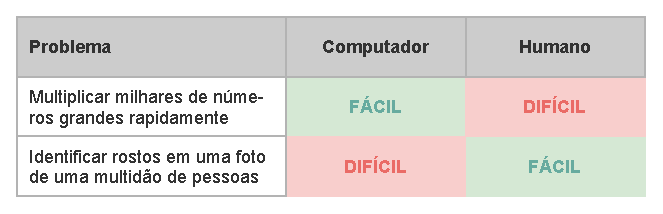
\includegraphics[scale=1.1]{img/img-fundamentacao-dificuldades.pdf}
  \label{fig:fund-dificuldades}
  \indentedfont[15.2cm]{Adaptado de \citeonline{ref:Rashid}}
\end{figure}

A Inteligência Artificial engloba a área de estudo do Aprendizado de Máquina, que por sua vez englobam as áreas do Aprendizado de Representação e Aprendizado Profundo, conforme o diagrama de Venn apresentado na \autoref{fig:fund-ia}.

\begin{figure}[h!] %H
  \centering
  \caption{Diagrama de Venn da Inteligência Artificial e suas áreas de estudo. }
  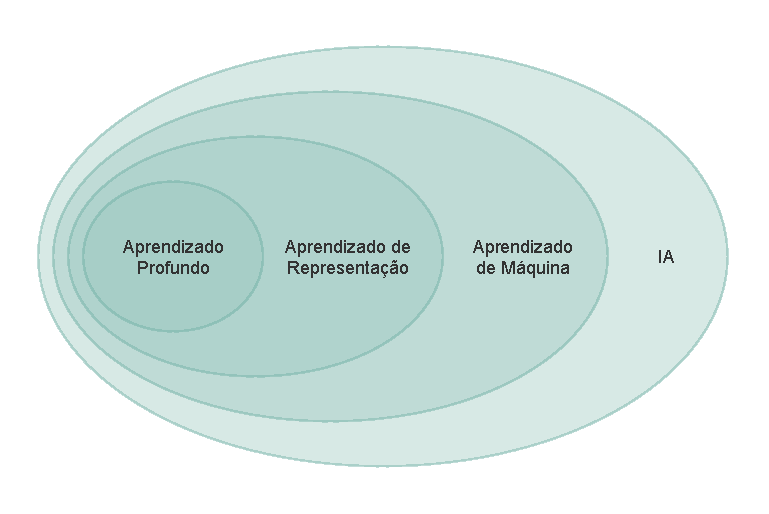
\includegraphics[scale=1.1]{img/img-fundamentacao-ia.pdf}
  \label{fig:fund-ia}
  \indentedfont[15.2cm]{Adaptado de \citeonline{ref:Goodfellow-Bengio-Courville}}
\end{figure}

Para evidenciar as diferenças entre essas áreas de estudo, em comparação com simples Sistemas Baseados em Regras, \citeonline{ref:Goodfellow-Bengio-Courville} apresenta um fluxograma com as etapas de processamento entre a entrada e a saída de dados para cada uma delas, presente na \autoref{fig:fund-fluxograma}.

\begin{figure}[h!] %H
  \centering
  \caption{Fluxograma que diferencia as áreas de estudo da Inteligência Artificial e suas etapas de processamento de dados. }
  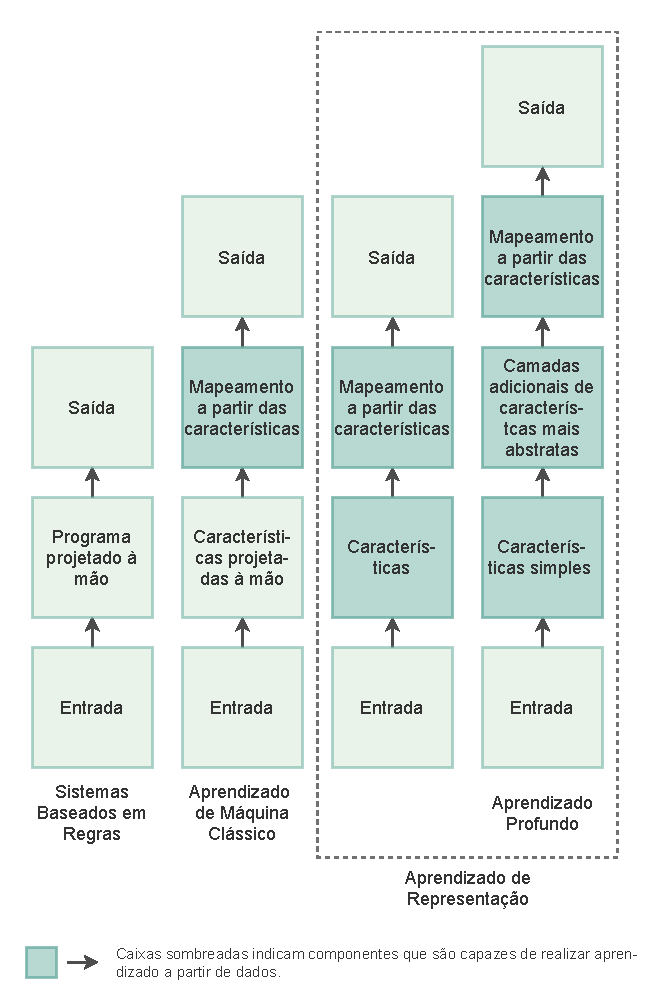
\includegraphics[scale=1.1]{img/img-fundamentacao-fluxograma.pdf}
  \label{fig:fund-fluxograma}
  \indentedfont[15.2cm]{Adaptado de \citeonline{ref:Goodfellow-Bengio-Courville}}
\end{figure}

Sistemas Baseados em Regras não possuem componentes capazes de realizar qualquer aprendizado a partir e dados \cite{ref:Goodfellow-Bengio-Courville} e são utilizados para resolução de problemas e/ou execução de tarefas que podem ser descritos por uma lista de regras formais, como por exemplo jogar Xadrez. Ao contrários desses sistemas, o Aprendizado de Máquina (do inglês \textit{Machine Learning}) utiliza algoritmos computacionais para transformar características reunidas empiricamente por cientistas de dados em modelos utilizáveis \cite{ref:Edgar-Manz} \cite{ref:Robins} possuindo a capacidade ``de se aprimorar [...], aprendendo novos conhecimentos ao invés de serem programado com eles'' \cite{ref:Woolf}.

No Aprendizado de Representação (do inglês \textit{Feature Learning} ou \textit{Representation Learning}) entretanto, não há necessidade de mapear manualmente essas características \cite{ref:Goodfellow-Bengio-Courville}. Ou seja, por conta própria e de forma abstrata, os algoritmos são capazes de extrair as características importantes para a construção dos modelos utilizando redes neurais \cite{ref:Robins} \cite{ref:Lesort}. O Aprendizado Profundo, por sua vez, resolve a dificuldade que o Aprendizado de Representação possui de extrair características abstratas de alto nível, tais como sotaques de um locutor \cite{ref:Goodfellow-Bengio-Courville}. Segundo \citeonline{ref:Mao-Wang-Tang-Qian}, o Aprendizado Profundo ``imita a função que o cérebro humano possui de interpretar dados usando redes neurais de várias camadas''. Um exemplo dessas variadas camadas é apresentado na \autoref{fig:fund-camadas}, onde características distintas são extraídas por cada camada. Uma comparação com o modelo de Aprendizado de Máquina é ilustrado na \autoref{fig:fund-aprendizados}.

\begin{figure}[h!] %H
  \centering
  \caption{Ilustração das camadas de um modelo de Aprendizado Profundo.}
  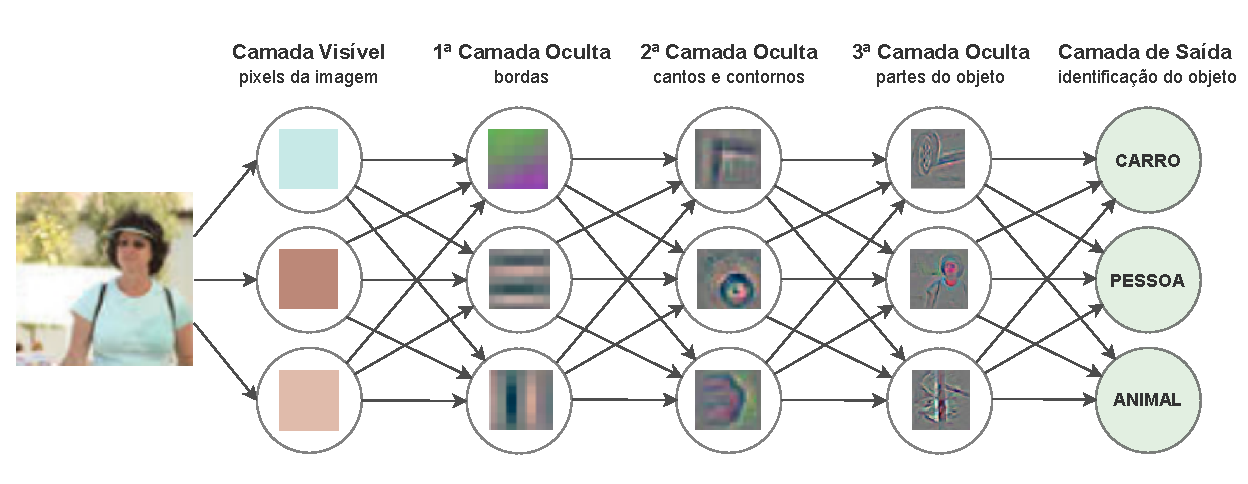
\includegraphics[scale=0.8]{img/img-fundamentacao-deep-learning.pdf}
  \label{fig:fund-camadas}
  \indentedfont[15.2cm]{Adaptado de \citeonline{ref:Goodfellow-Bengio-Courville}}
\end{figure}

\begin{figure}[h!] %H
  \centering
  \caption{Comparação entre os modelos Aprendizado de Máquina e Aprendizado Profundo.}
  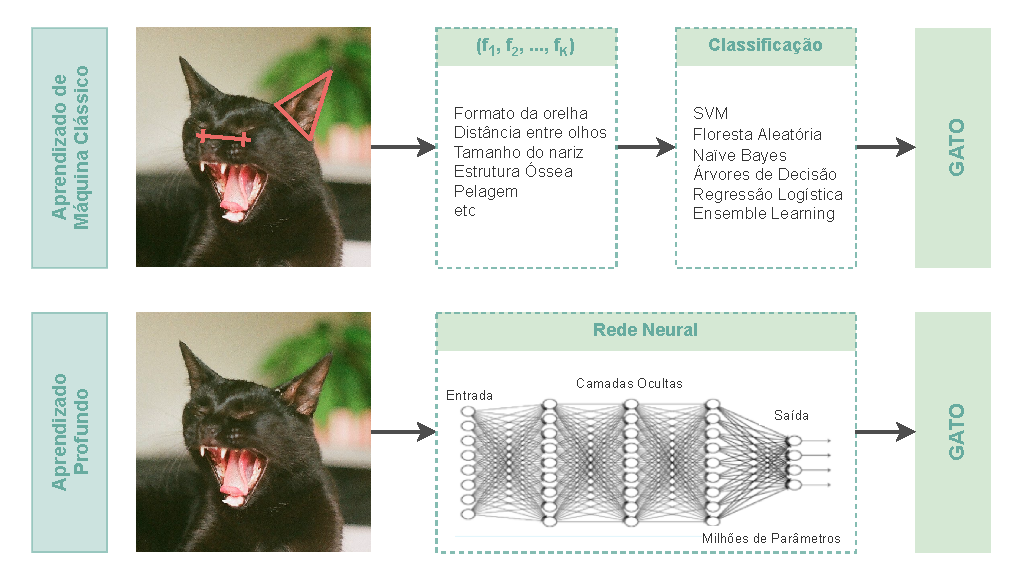
\includegraphics[scale=0.95]{img/img-fundamentacao-aprendizados.pdf}
  \label{fig:fund-aprendizados}
  \indentedfont[15.2cm]{Adaptado de \citeonline{ref:Robins}}
\end{figure}

\subsection{Redes Neurais} \label{cap:fund-ia-rn}
Ao contrário da abordagem convencional de programação, onde dizemos a um computador o que deve ser feito ao dividir um problema em pequenas tarefas para que ele execute, uma Rede Neural (do inglês \textit{Neural Network}) utiliza dados observacionais para aprender como resolver o problema \cite{ref:Nielsen}.

\citeonline{ref:Walczak-Cerpa} define Redes Neurais Artificiais como modelos que ``simulam a atividade elétrica do cérebro e do sistema nervoso''. Porém enquanto alguns tipos de redes neurais tem sido utilizadas para entender o funcionamento do cérebro, na perspectiva de Aprendizado Profundo elas não são projetadas para serem modelos realistas da função biológica \cite{ref:Goodfellow-Bengio-Courville}.

Uma Rede Neural é composta por camadas de nós, conhecidos como neurônios, e conexões que interligam as saídas e entradas desses nós. A estrutura básica de uma Rede Neural é ilustrada na \autoref{fig:fund-nn}, onde a primeira camada de neurônios é a camada de entrada, a última camada é a camada de saída e as camadas entre elas são chamadas de camadas ocultas. Na \autoref{fig:fund-nn}, vetor $\mathrm{X}$ contém os valores de entrada, os vetores $\mathrm{a^{[l]}}$ representam as funções de ativação referentes à \textit{l-ésima} camada, e $\mathrm{\hat{y}}$ é o vetor de saída com os valores preditos. Essas notações estão de acordo com as propostas por \citeonline{ref:Ng} presentes no \autoref{apendice:notacao}.

\begin{figure}[h!] %H
  \centering
  \caption{Estrutura básica de uma Rede Neural com duas camadas.}
  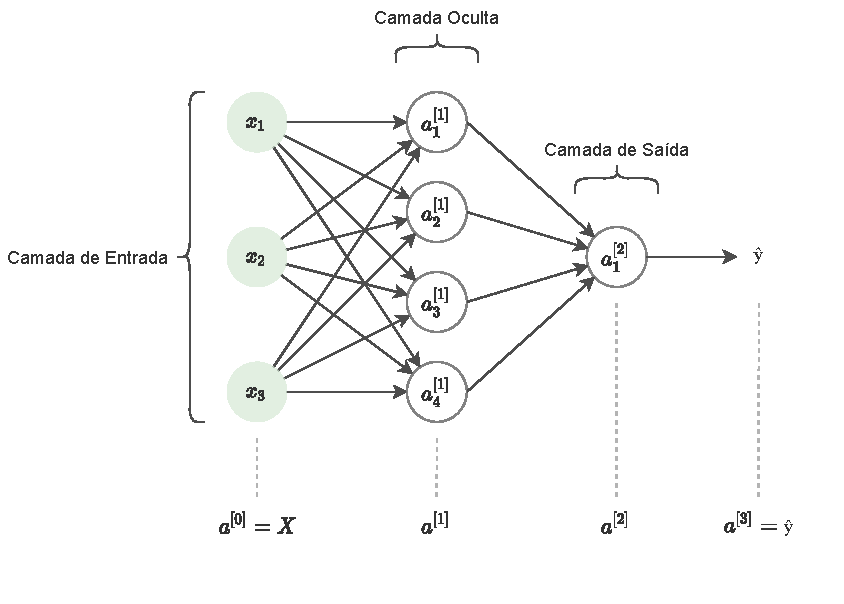
\includegraphics[scale=1.1]{img/img-fundamentacao-nn.pdf}
  \label{fig:fund-nn}
  \indentedfont[15.2cm]{Autoria própria}
\end{figure}



São nos neurônios que ocorrem as computações. Eles são responsáveis por combinar a entrada de dados com um conjunto de pesos que as amplificam ou as amortecem \cite{ref:Nicholson}. A \autoref{fig:fund-no} mostra um diagrama de um nó de uma Rede Neural.

\begin{figure}[h!] %H
  \centering
  \caption{Diagrama de um Neurônio de uma Rede Neural.}
  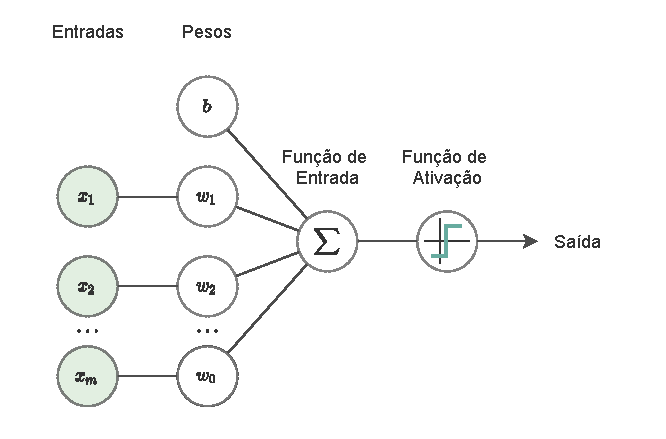
\includegraphics[scale=1.1]{img/img-fundamentacao-no.pdf}
  \label{fig:fund-no}
  \indentedfont[15.2cm]{Adaptado de \citeonline{ref:Nicholson}}
\end{figure}

\subsubsection{Funções de Ativação} \label{cap:fund-ia-rn-func}

% In the conventional approach to programming, we tell the computer what to do, breaking big problems up into many small, precisely defined tasks that the computer can easily perform. By contrast, in a neural network we don’t tell the computer how to solve our problem. Instead, it learns from observational data, figuring out its own solution to the problem at hand.

%While the kinds of neural networks used for machine learning have sometimes been used to understand brain function (Hinton and Shallice, 1991), they are generally not designed to be realistic models of biological function. The neural perspective on deep learning is motivated by two main ideas. One idea is that the brain provides a proof by example that intelligent behavior is possible, and a conceptually straightforward path to building intelligence is to reverse engineer the computational principles behind the brain and duplicate its functionality. Another perspective is that it would be deeply interesting to understand the brain and the principles that underlie human intelligence, so machine learning models that shed light on these basic scientific questions are useful apart from their ability to solve engineering applications.

%ANN models simulate the electrical activity of the brain and nervous system. Processing elements (also known as either a neurode or perceptron) are connected to other processing elements. Typically the neurodes are arranged in a layer or vector, with the output of one layer serving as the input to the next layer and possibly other layers. A neurode may be connected to all or a subset of the neurodes in the subsequent layer, with these connections simulating the synaptic connections of the brain.


%Segundo \citeonline{ref:Goodfellow-Bengio-Courville}, a Inteligência Artificial (IA) em seus primórdios foi muito utilizada para resolução de problemas matemáticos que são complexos para seres humanos, porém simples para computadores. Porém, ainda segundo \citeonline{ref:Goodfellow-Bengio-Courville}, o verdadeiro desafio da IA atualmente é resolver problemas que na verdade são tarefas simples para pessoas mas complexas para computadores, como fazer o reconhecimento de fala ou rostos em fotos.

%Porém apenas recentemente houveram avanços em pesquisas permitindo com que as habilidades de computadores fossem igualadas as do seres humanos em tarefas mais corriqueiras, como reconhecimento de objetos e de fala.

%Tarefas mais abstratas que podem ser descritas por uma lista de regras formais como jogar xadrez, ao contrário de tarefas mais corriqueiras como reconhecimento de objetos, onde avanços nas pesquisas foram obtidos apenas recentemente permitindo igualar habilidades humanas com as de computadores.


%\section{Aprendizagem Profunda} \label{cap:fund-aprendizagem}

%\section{Redes Neurais Profundas} \label{cap:fund-redes_profundas}

%\section{Redes Neurais Convolucionais} \label{cap:fund-redes_convolucionais}

%\section{Frameworks e Bibliotecas} \label{cap:fund-frameworks}

%    \subsection{OpenCV} \label{cap:fund-frameworks-opencv}

%    \subsection{Darknet} \label{cap:fund-frameworks-darknet}

%    \subsection{Flask} \label{cap:fund-frameworks-flask}


\begin{comment}


\end{comment}
